\section{Simulation}
\label{sec:simulation}

Simulation provides both a proof of concept for the \(R_{e/\mu}\) analysis and
a first implementation of reconstruction methods intended to run on
experimental data. The same reconstruction chain should be usable after either
simulated events have been transported through detector-response models or real
events have been converted into the same detector-level data products. For
Phase I, the primary production mode is stopped \(\pi^+\) decay, but the
Geant4 stage can also be configured for targeted studies of detector geometry,
beam conditions, material effects, and specific event topologies. The practical
requirement is that the analysis strategy should work on detector-level
observables, with modeled detector response, before it is applied to data
\cite{schwendimann_framework_status_2025,carlton_annual_update_2026}.

\subsection{End-to-End Software Chain}
\label{subsec:simulation-software-chain}

The PIONEER simulation framework is organized as a sequence of replaceable
software stages. A geometry-building stage constructs the detector description
from configurable inputs, allowing detector concepts, local test setups, and
material studies to be changed without rewriting the full chain. A
Geant4-based Monte Carlo stage then generates the requested primary particles
or decays and transports particles through the detector material
\cite{geant4_2003,geant4_2016}. This stage also records truth-level
information, such as particle identities, trajectories, energy deposits, decay
points, and interaction volumes.

\begin{figure}[!htbp]
  \centering
  \begin{subfigure}{0.42\textwidth}
    \centering
    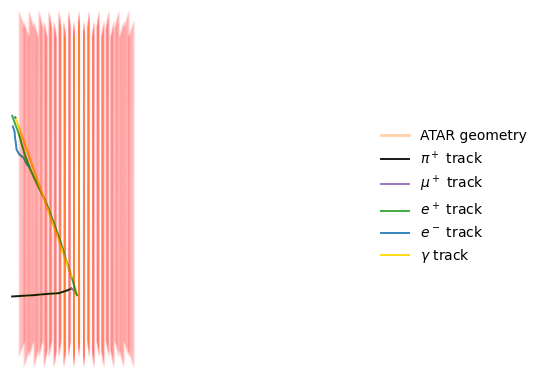
\includegraphics[width=\textwidth]{../resources/figures/chapters/01_introduction/atar_sim_render}
    \caption{ATAR side view}
  \end{subfigure}
  \hfill
  \begin{subfigure}{0.47\textwidth}
    \centering
    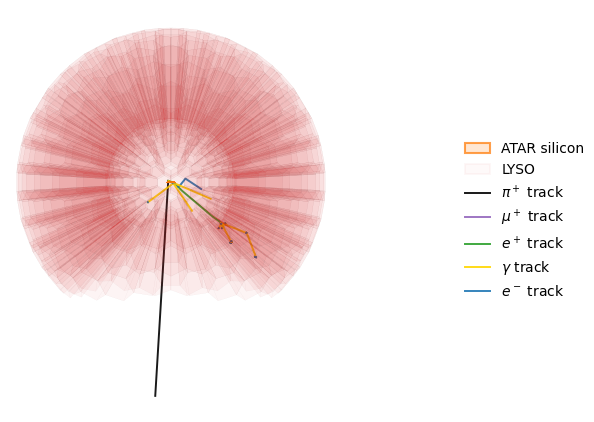
\includegraphics[width=\textwidth]{../resources/figures/chapters/01_introduction/lyso_sim_render}
    \caption{LYSO top-down view}
  \end{subfigure}
\caption{
Example simulated stopped-pion event displayed in the PIONEER detector
geometry. Panel (a) shows a side view of the active-target region containing
the incoming pion, short muon segment, and outgoing decay products near the
pion stopping point. Panel (b) shows the same event projected onto the
transverse plane of the LYSO calorimeter, illustrating the corresponding
distribution of activity throughout the calorimeter array. Together, the two
views demonstrate how particle trajectories and detector response are
represented within the simulation framework.
}
  \label{fig:simulation-geometry-renders}
\end{figure}

The detector-response and reconstruction stages are implemented in the Gaudi
framework, which provides a configurable event-processing pipeline used widely
in high-energy physics \cite{gaudi_2001}. Detector response converts simulated
energy deposits and truth information into ROOT-based detector data structures.
Reconstruction then consumes these detector-level objects and produces
analysis quantities such as positron energy, time, and angle; pion-stop
observables; ATAR event classifications; calorimeter clusters; and
event-summary objects
\cite{reconstruction_overview_2025,schwendimann_framework_status_2025}.

This staged structure encourages modular detector R\&D and isolated studies.
Geometry, response, or reconstruction stages can be replaced, removed, or
specialized to determine how a particular assumption affects later analysis
quantities. The project is distributed with a Docker-based environment and
configurable production workflows so that simulation campaigns can be rerun
reproducibly as detector descriptions and reconstruction methods are updated.

\subsection{Detector Response and Reconstruction}
\label{subsec:simulation-reconstruction}

The detector-response stage converts idealized Monte Carlo information into
observables limited by detector resolution, thresholds, timing, segmentation,
inactive material, and pileup. These effects are essential because the
experimental challenges are not set by two-body decay kinematics alone. For
example, calorimeter response studies can include energy and timing
resolution, shower leakage, low-energy response tails, and nearby-pulse
separation. ATAR response studies can convert simulated energy deposits into
strip-level hit information with modeled position, time, and energy
resolution. As test-beam data become available, detector-response models can
be tied to measured performance rather than only to idealized assumptions
\cite{reconstruction_overview_2025,lyso_calo_intro_2025}.

Reconstruction is developed in parallel with the detector-response model. For
the ATAR, the observable-based chain can be described schematically as
tracklet finding, tracklet fitting, pattern finding, and event classification.
Tracklet finding groups nearby hits in space and time; fitting estimates local
trajectories and endpoints; pattern finding associates reconstructed objects
with a physics hypothesis such as a direct \(\pi\to e\nu\) decay or a
sequential \(\pi\to\mu\to e\) chain. Calorimeter reconstruction provides
positron energy, time, and position information, while tracker information may
provide an additional direction or matching constraint if it is included in the
final detector design \cite{reconstruction_overview_2025}.

\begin{figure}[!htbp]
  \centering
  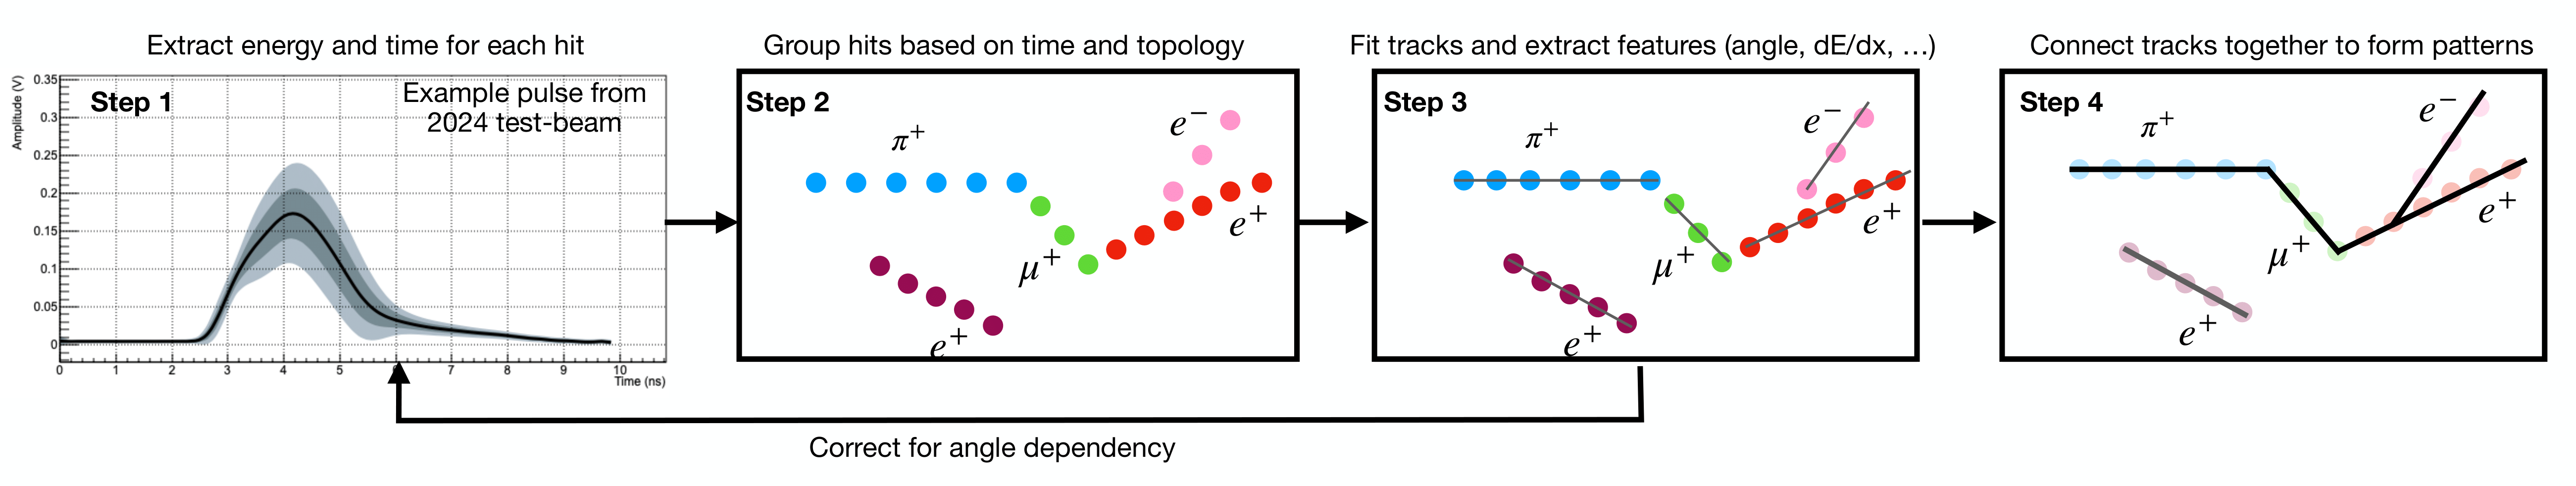
\includegraphics[width=\textwidth]{../resources/figures/chapters/01_introduction/atar_reco_algo-1}
  \caption{
  Conceptual ATAR reconstruction workflow. Waveform pulses are converted into
  time- and energy-calibrated hits, grouped into candidate particle segments,
  fit to extract track-level features, and finally associated into event-level
  topology hypotheses. The resulting patterns can be used to identify pion
  stops, muon tracks, positrons, and background topologies relevant to the
  \(R_{e/\mu}\) measurement.
  }
  \label{fig:atar-reconstruction-chain}
\end{figure}

A useful feature of the framework is the distinction between truth-guided and
observable-based reconstruction. Truth-guided reconstruction uses Monte Carlo
information to diagnose what an ideal algorithm could recover, to define
targets, and to locate the origin of failures. Observable-based reconstruction
uses only detector quantities that would be available in data. The goal is not
to make the analysis depend on truth, but to use truth during development to
understand biases, inefficiencies, and topology-dependent failures before
transitioning to data-like reconstruction
\cite{schwendimann_framework_status_2025,carlton_annual_update_2026}.

\subsection{Machine-Learning Interface}
\label{subsec:simulation-ml-interface}

Machine-learning reconstruction uses the same simulation chain but adds an
interface between detector response and model training. A Gaudi algorithm
writes ML-ready parquet datasets containing detector-response objects together
with optional truth targets. This allows the simulation to provide both the
inputs that a model would see in data and the labels needed for supervised
training. The separate \texttt{pioneerML} framework then handles
model-specific data loading, preprocessing, training, evaluation, and
inference through a plugin-based workflow.

The ATAR is a natural target for graph-based learning because each event is a
set of sparse strip hits with geometry, timing, and energy information. The
\texttt{pioneerML} framework is intended to support multiple appended
reconstruction models rather than a single fixed architecture. As one example,
the plugin housing the PURITY model can form graph representations from event
data, supply nodes carrying hit features such as position, view, time, and
deposited energy, and optionally include calorimeter information. Similar
plugins can target tasks such as classification, pattern finding, endpoint
regression, pion-stop regression, or positron-angle estimation. In this sense,
the ML framework does not replace the simulation; it appends to it, using
simulated truth to bootstrap reconstruction methods that can later be compared
with, or combined with, rule-based algorithms
\cite{carlton_annual_update_2026,reconstruction_overview_2025}.

\subsection{Simulation Challenges}
\label{subsec:simulation-challenges}

The main simulation challenge is that the analysis precision is driven by rare
failures. The dominant \(\pi\to\mu\to e\) chain is roughly four orders of
magnitude more common than the direct \(\pi\to e\nu\) decay, so small
misidentification probabilities can matter. The simulation must therefore
stress-test difficult topologies, including low-energy positrons that scatter
or annihilate in the ATAR, pion or muon decays in flight, accidental activity
from old muon decays, positrons emitted near detector regions with reduced
angular information, and calorimeter-tail events that move across the analysis
threshold.

\begin{figure}[!htbp]
  \centering
  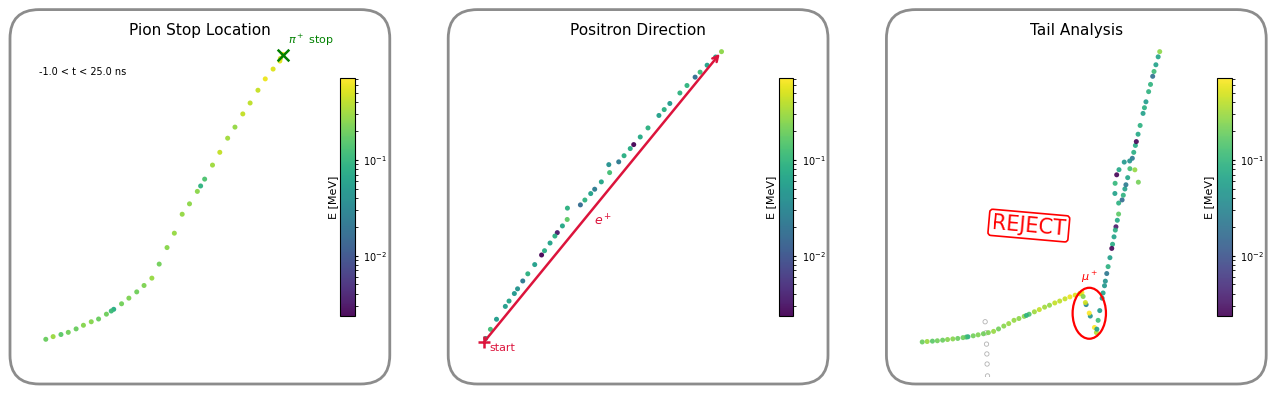
\includegraphics[width=0.95\textwidth]{../resources/figures/chapters/01_introduction/simulation_difficulties}
  \caption{
  Example ATAR reconstruction tasks relevant to the \(R_{e/\mu}\)
  measurement. Left: determination of the pion stopping location from the
  three-dimensional energy-deposition pattern. Center: reconstruction of the
  outgoing positron direction from sparse tracker hits. Right: identification and
  rejection of events containing visible muon activity, which can contaminate
  samples used to characterize the low-energy \(\pi\to e\nu\) response tail.
  }
  \label{fig:simulation-difficult-topologies}
\end{figure}

These studies are iterative. A simulation production exposes a failure mode;
the detector-response model, reconstruction algorithm, or selection strategy
is modified; and the chain is rerun to determine whether the change removes a
physics bias or only improves an intermediate metric. This feedback loop is
the reason the framework is organized around replaceable geometry, response,
and reconstruction stages. The purpose of the simulation section in this
dissertation is therefore to define the tools and assumptions used in later
chapters, not to present the final sensitivity result.

\FloatBarrier
